\parindent=0em
% El comando "\chp" es como el "\chapter" pero mete "Chapter" en vez de "Capitulo"
\chp{1}{Introduction}

% addtocounter: necesario para tener el mismo número de \section que el de español ==> -2 porque hay 2 secciones en el capitulo 9
\addtocounter{section}{-4}

\pagenumbering{arabic}
\noindent
% \texttt{Lorem ipsum dolor sit amet, consectetuer ad}\\
This chapter will explain the motivation, objectives, work structure and work planning for this project.

\section{Motivation}
% When a person decides to perform any activity with the aim of improving their physical condition, either by increasing or decreasing their weight, they realize that one of the most important factors in achieving this goal is the planning of a healthy and balanced diet.

% For this purpose, complementary tools can be used to carry out this planning, to follow a balanced diet and to plan the different meals during the day.

% With the aim of helping all these users, it has been decided to develop an Android application, in which users will be allowed to follow other diets created. Using this application, the user's eating habits can be improved, keeping a count of calories consumed, understanding food labeling, consulting the nutritional information of the food or even elaborating diets to help the rest of the users.

% introducir el dominio
Every athlete needs to accompany his or her activity with an adequate diet, since nutrition is one of the factors on which physical performance depends. An adequate diet provides the necessary nutrients to maintain an optimal state of health, which translates into performance. Depending on how an athlete eats, you can see how food affects their performance, improving performance and recovery, limiting or even decreasing them, as poor nutrition can promote injuries and fatigue.

% plantear el problema
Currently, there are no mobile applications that can flexibly manage the diets that an athlete needs to follow in order to have a healthy diet that is appropriate to his or her profile. In addition, most of the existing diets on the Internet lack sources or studies that support them and do not have reliable feedback from users who have tried them.

% propuesta que planteamos
To solve these limitations, it has been decided to create an Android application that meets the needs of monitoring and control of diets. It is also possible to see the feedback of the athletes who have followed and evaluated the diet, playing the role of a social network and helping other athletes who are looking for similar goals. In addition, athletes can attach documents to the diets to provide additional information to support them.
\section{Objectives}
The main objective of this project is to develop an Android application that helps athletes to complement their physical activity, following a healthy and balanced diet to achieve the desired physical shape. It is also possible to interact with other athletes, creating diets that can be followed by other athletes or including comments and evaluations in them.

More specific objectives can be defined based on the main objective:
\begin{itemize}
    \item Allow an athlete to register in the application to discover and analyze all the diets in the application, and to update the weight and insert the daily steps, in order to keep a tally and visualize the progress in graphs.
    \item Allow athletes to follow a diet inserted from the application by any of the users, whether they are athletes or administrators.
    \item To offer the possibility to the athlete to evaluate the diet he/she is following, in order to help other athletes to decide and know which diets are being effective.
    \item Allow all athletes the ability to create one or more diets, detailing the foods that compose it, the recommended amount of each one of them and even publishing documentation that helps to follow the diet.
    \item Allow athletes to add foods to diets and have their nutritional information updated at all times.
\end{itemize}
\section{Organización de la memoria}
A continuación se describe de manera breve la estructura de la memoria:

\begin{itemize}
    \item \textbf{Capítulo 1:} en este capítulo se describe la motivación del trabajo, los objetivos y la estructura de la memoria.
    \item \textbf{Capítulo 2:} en este capítulo se estudian herramientas similares a la que se ha realizado en el trabajo.
    \item \textbf{Capítulo 3:} en este capítulo se describe la tecnología utilizada para implementar el proyecto.
    \item \textbf{Capítulo 4:} en este capítulo se definen los actores y casos de uso que se explicarán mediante tablas junto a sus requisitos.
    \item \textbf{Capítulo 5:} en este capítulo se explica el diagrama entidad relación en el que se ha basado el proyecto y la implementación de la base de datos.
    \item \textbf{Capítulo 6:} en este capítulo se explica la arquitectura de la aplicación y los patrones utilizados.
    \item \textbf{Capítulo 7:} en este capítulo se realiza un estudio sobre el diseño e implementación de los casos de uso más relevantes.
    \item \textbf{Capítulo 8:} en este capítulo se exponen las estadísticas aportadas por usuarios que han dado su opinión sobre el producto.
    \item \textbf{Capítulo 9:} en este capítulo se enumeran los casos de uso que se harán en un futuro explicándolos brevemente.
    \item \textbf{Capítulo 10:} en este capítulo se expone el trabajo realizado por cada uno de los autores.
    \item \textbf{Anexo I:} manual de usuario.
    \item \textbf{Anexo II:} preguntas de evaluación.

\end{itemize}

\section{Planning}
This part describes all the planning carried out during the development of this project, detailing the different meetings and iterations performed. In figure  \ref{fig:gantt} the following \textbf{\textit{Gantt}} diagram can be seen where the different phases of the project are indicated.
\begin{figure}[H]
    \centering
    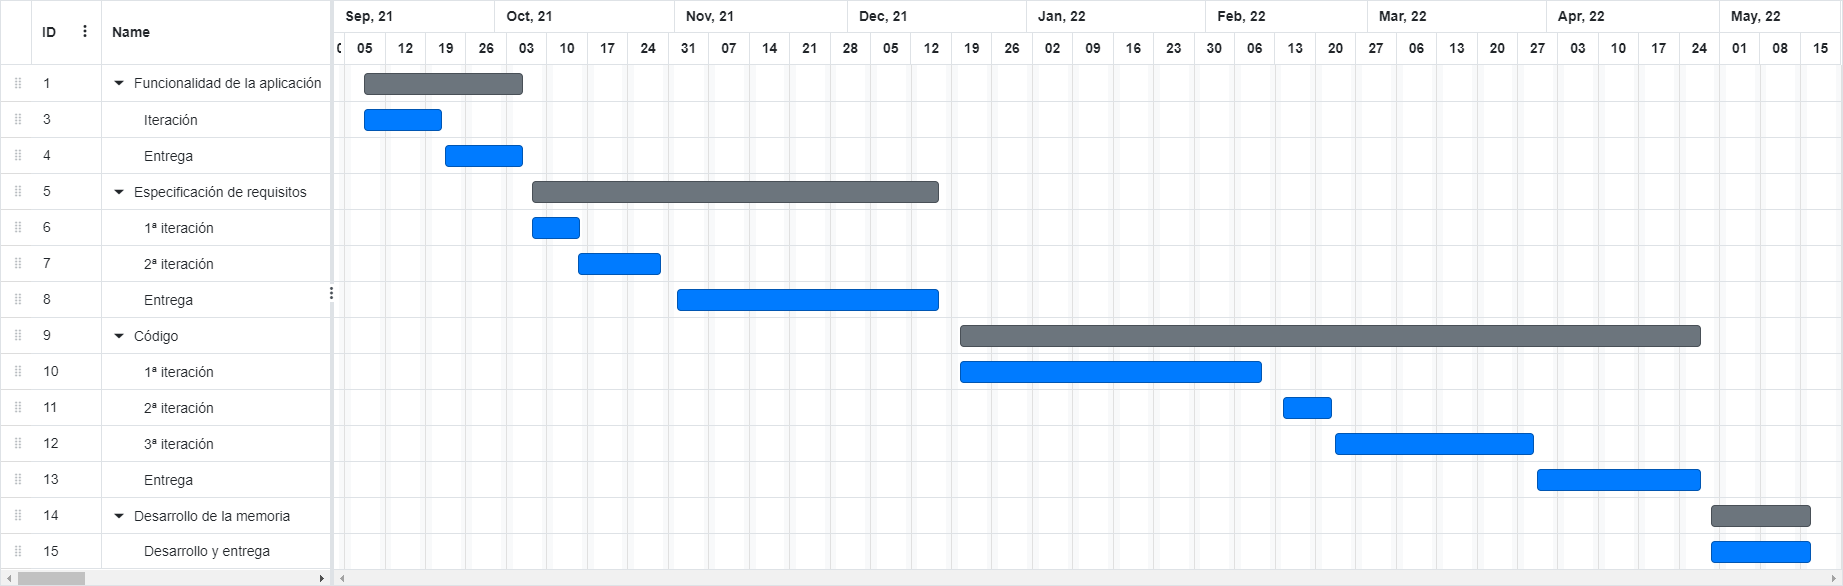
\includegraphics[width=\textwidth]{Images/gantt.png}
    \caption{Gantt chart of project planning}
    \label{fig:gantt}
\end{figure}

During the first phase, the main functionalities of the application were established. Once this phase was completed, the requirements were specified as well as the actors and modules that make up the application. Two iterations were carried out in order to establish the final requirements.

Subsequently, three code iterations were established, in each of which the different modules previously established (login, diet, current diet) were developed. After the code iterations, different white box tests were performed on the different use cases. In the last phase, the memory that complements the code was developed.

In order to carry out the different phases mentioned above, the team held meetings every Saturday, in order to establish the functionality to be developed during the week. At the same time, the meetings helped to know what the team members had done during the previous week, as well as to try to solve together the problems that arose.